\documentclass{scrarticle}
\usepackage[
%showframe,
left=2cm,
right=2cm,
top=2cm,
bottom=2cm
]{geometry} %Layout des Dokuments
\usepackage{graphicx}
\usepackage{amsmath}
\usepackage{hyperref}
\begin{document}
	%---------------Erklärung-------------------
	%[h!hbt] -> Erzwingung der Position der Graphik (b = buttom, t = top, h! = here (Gezwungen und ignoriert Latex-Automatisierungen), h = here)
	%[width=XX\linewidth] -> Größe an die Zeilenlänge anpassen
	%[height=XX\textheight] -> Größe an die Seite anpassen !WENN IN NUTZUNG BEIDER GRÖßEN-VERÄNDERUNGEN!, alles in einer eckigen Klammer setzen und mit einem Kommata trennen (siehe Beispiel -> Image Größe anpassen) Es ist auch möglich spezifische Größen wie bspw. 0.5cm anzugeben.
	%\graphicspath{dir-list} -> Direkt-Anweisung, wo die Images liegen (In diesem Beispiel nicht genutzt, aber wäre Möglich.)
	
 	\section{Image einfügen}
	\begin{figure}[h!hbt]
		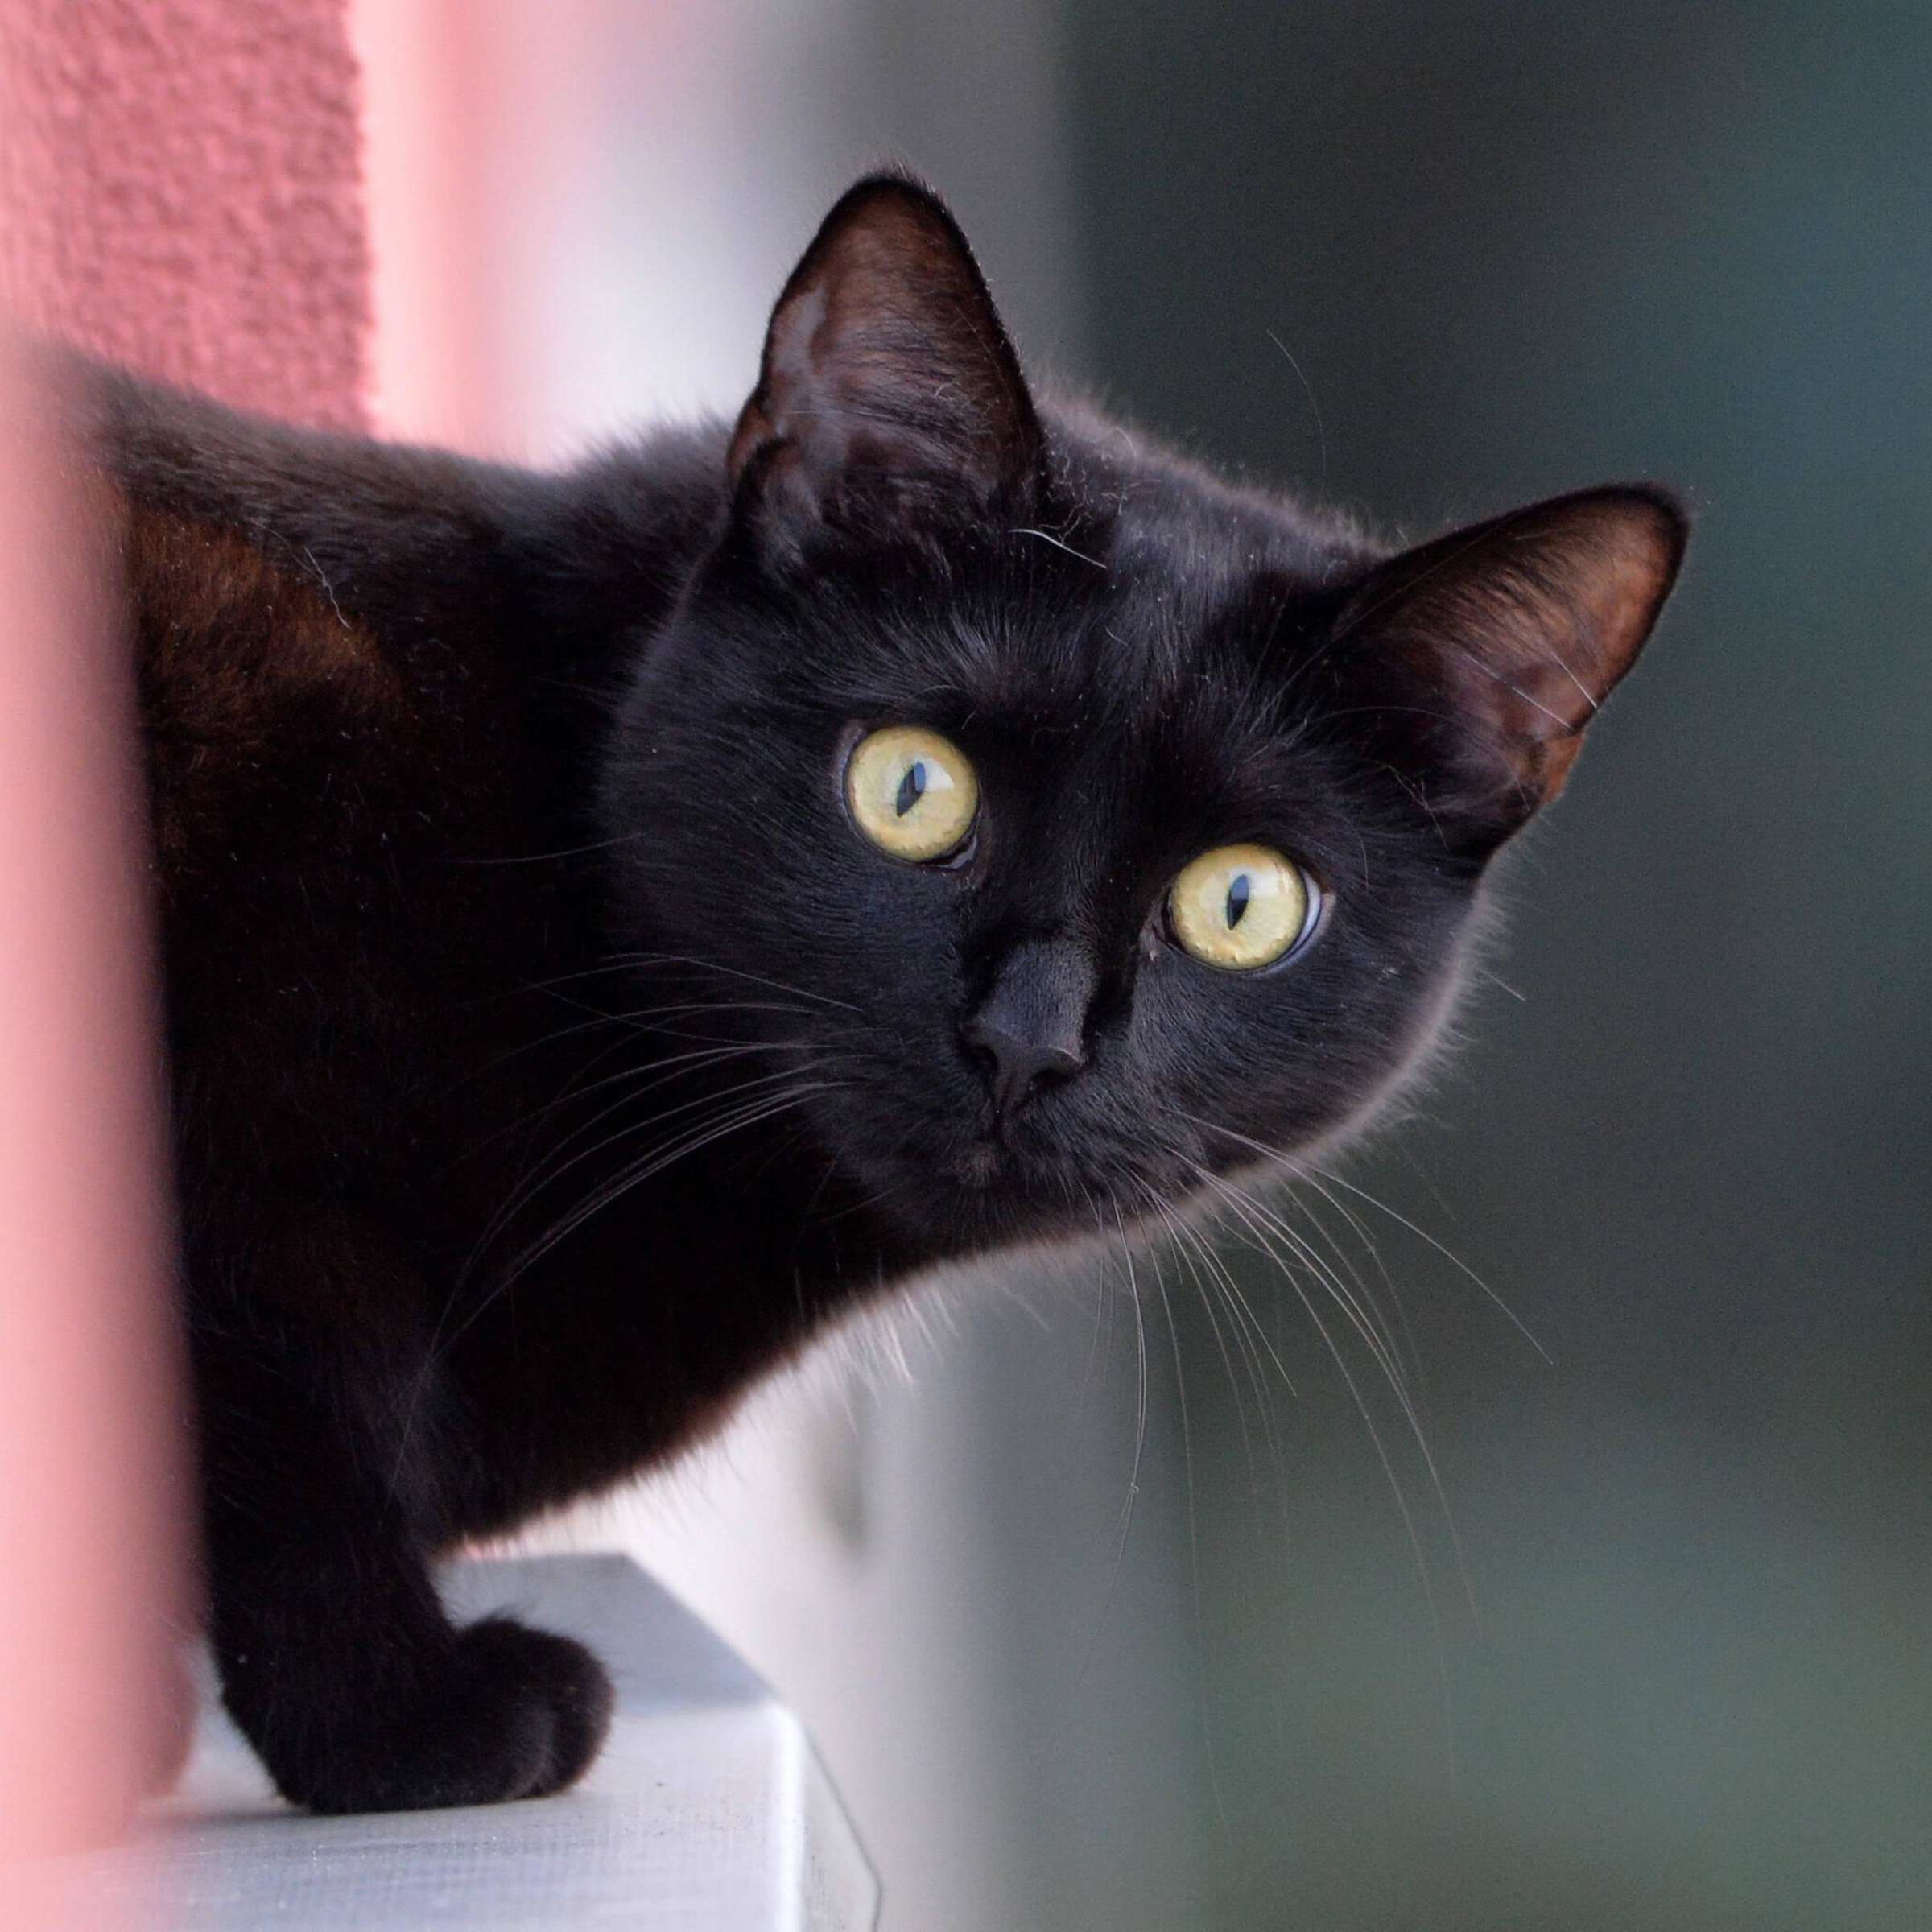
\includegraphics[width=\linewidth]{./Abbildungen/Beispiel.jpg}
	\end{figure}	
	\newpage
	
	\section{Image zentriert einfügen}
	\begin{figure}[h!hbt]
		\centering
		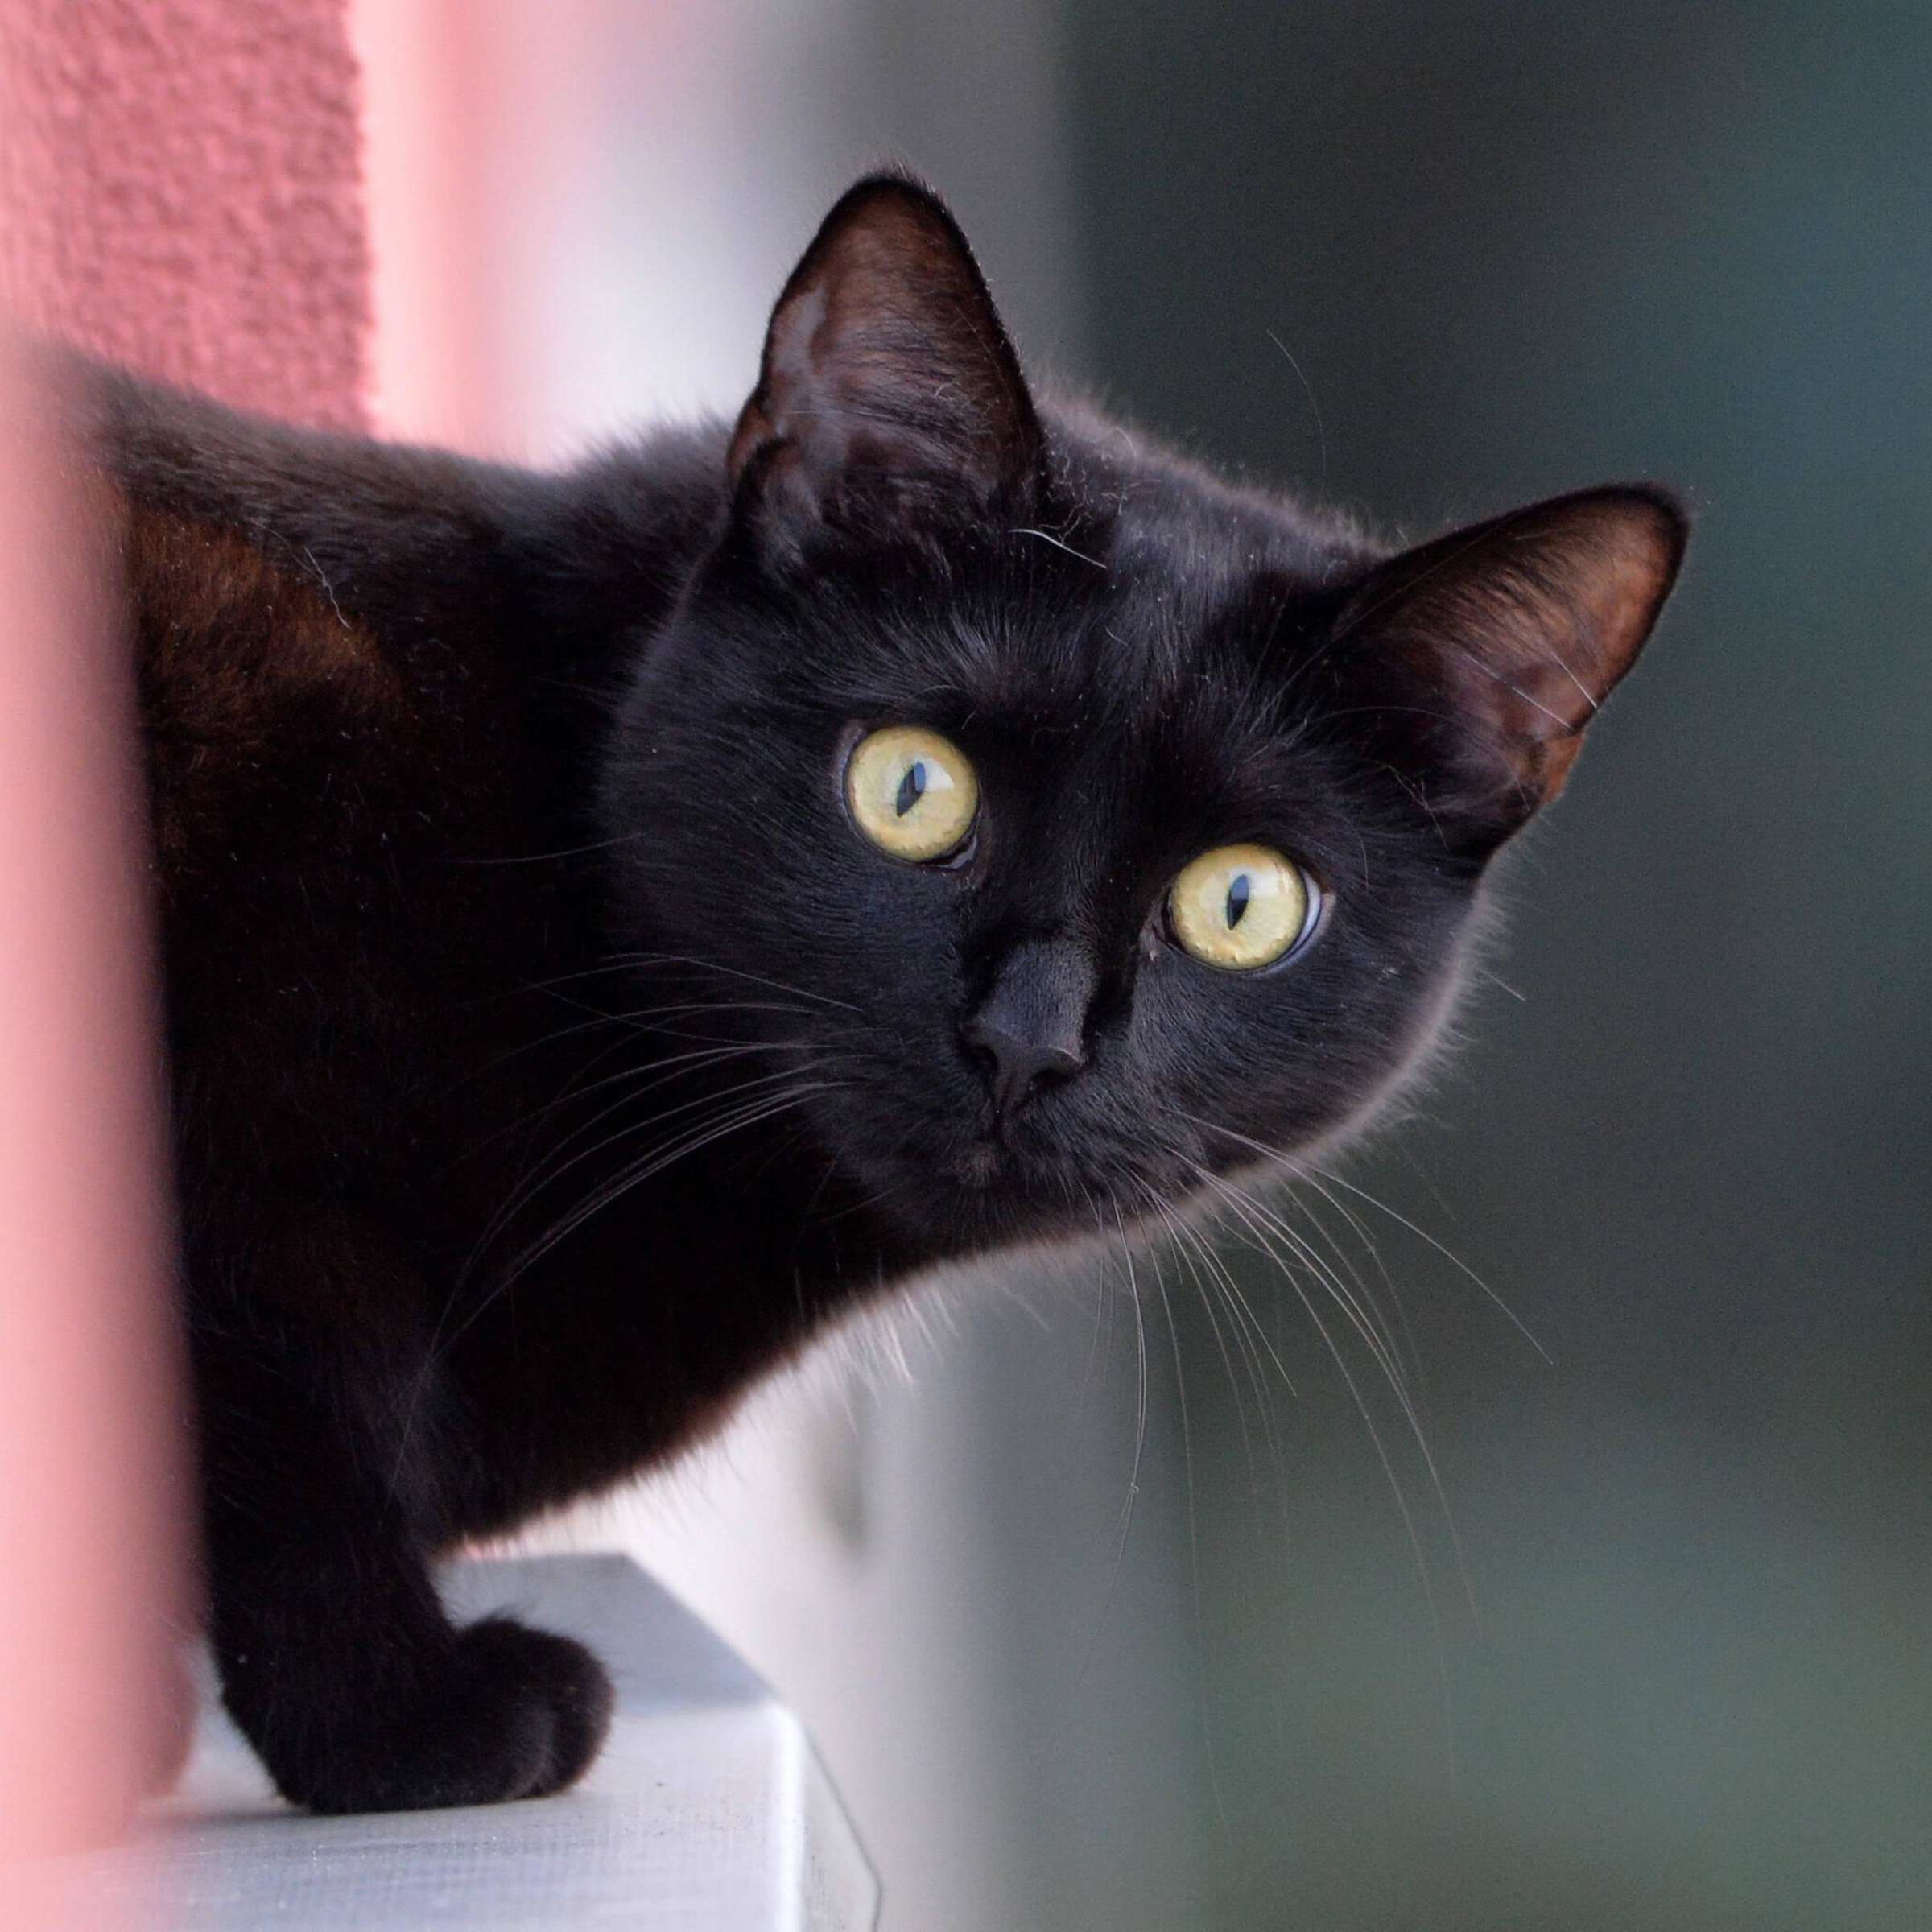
\includegraphics[width=\linewidth]{./Abbildungen/Beispiel.jpg}
	\end{figure}
	\newpage
	
	\section{Image Größe anpassen}
	\begin{figure}[h!hbt]
		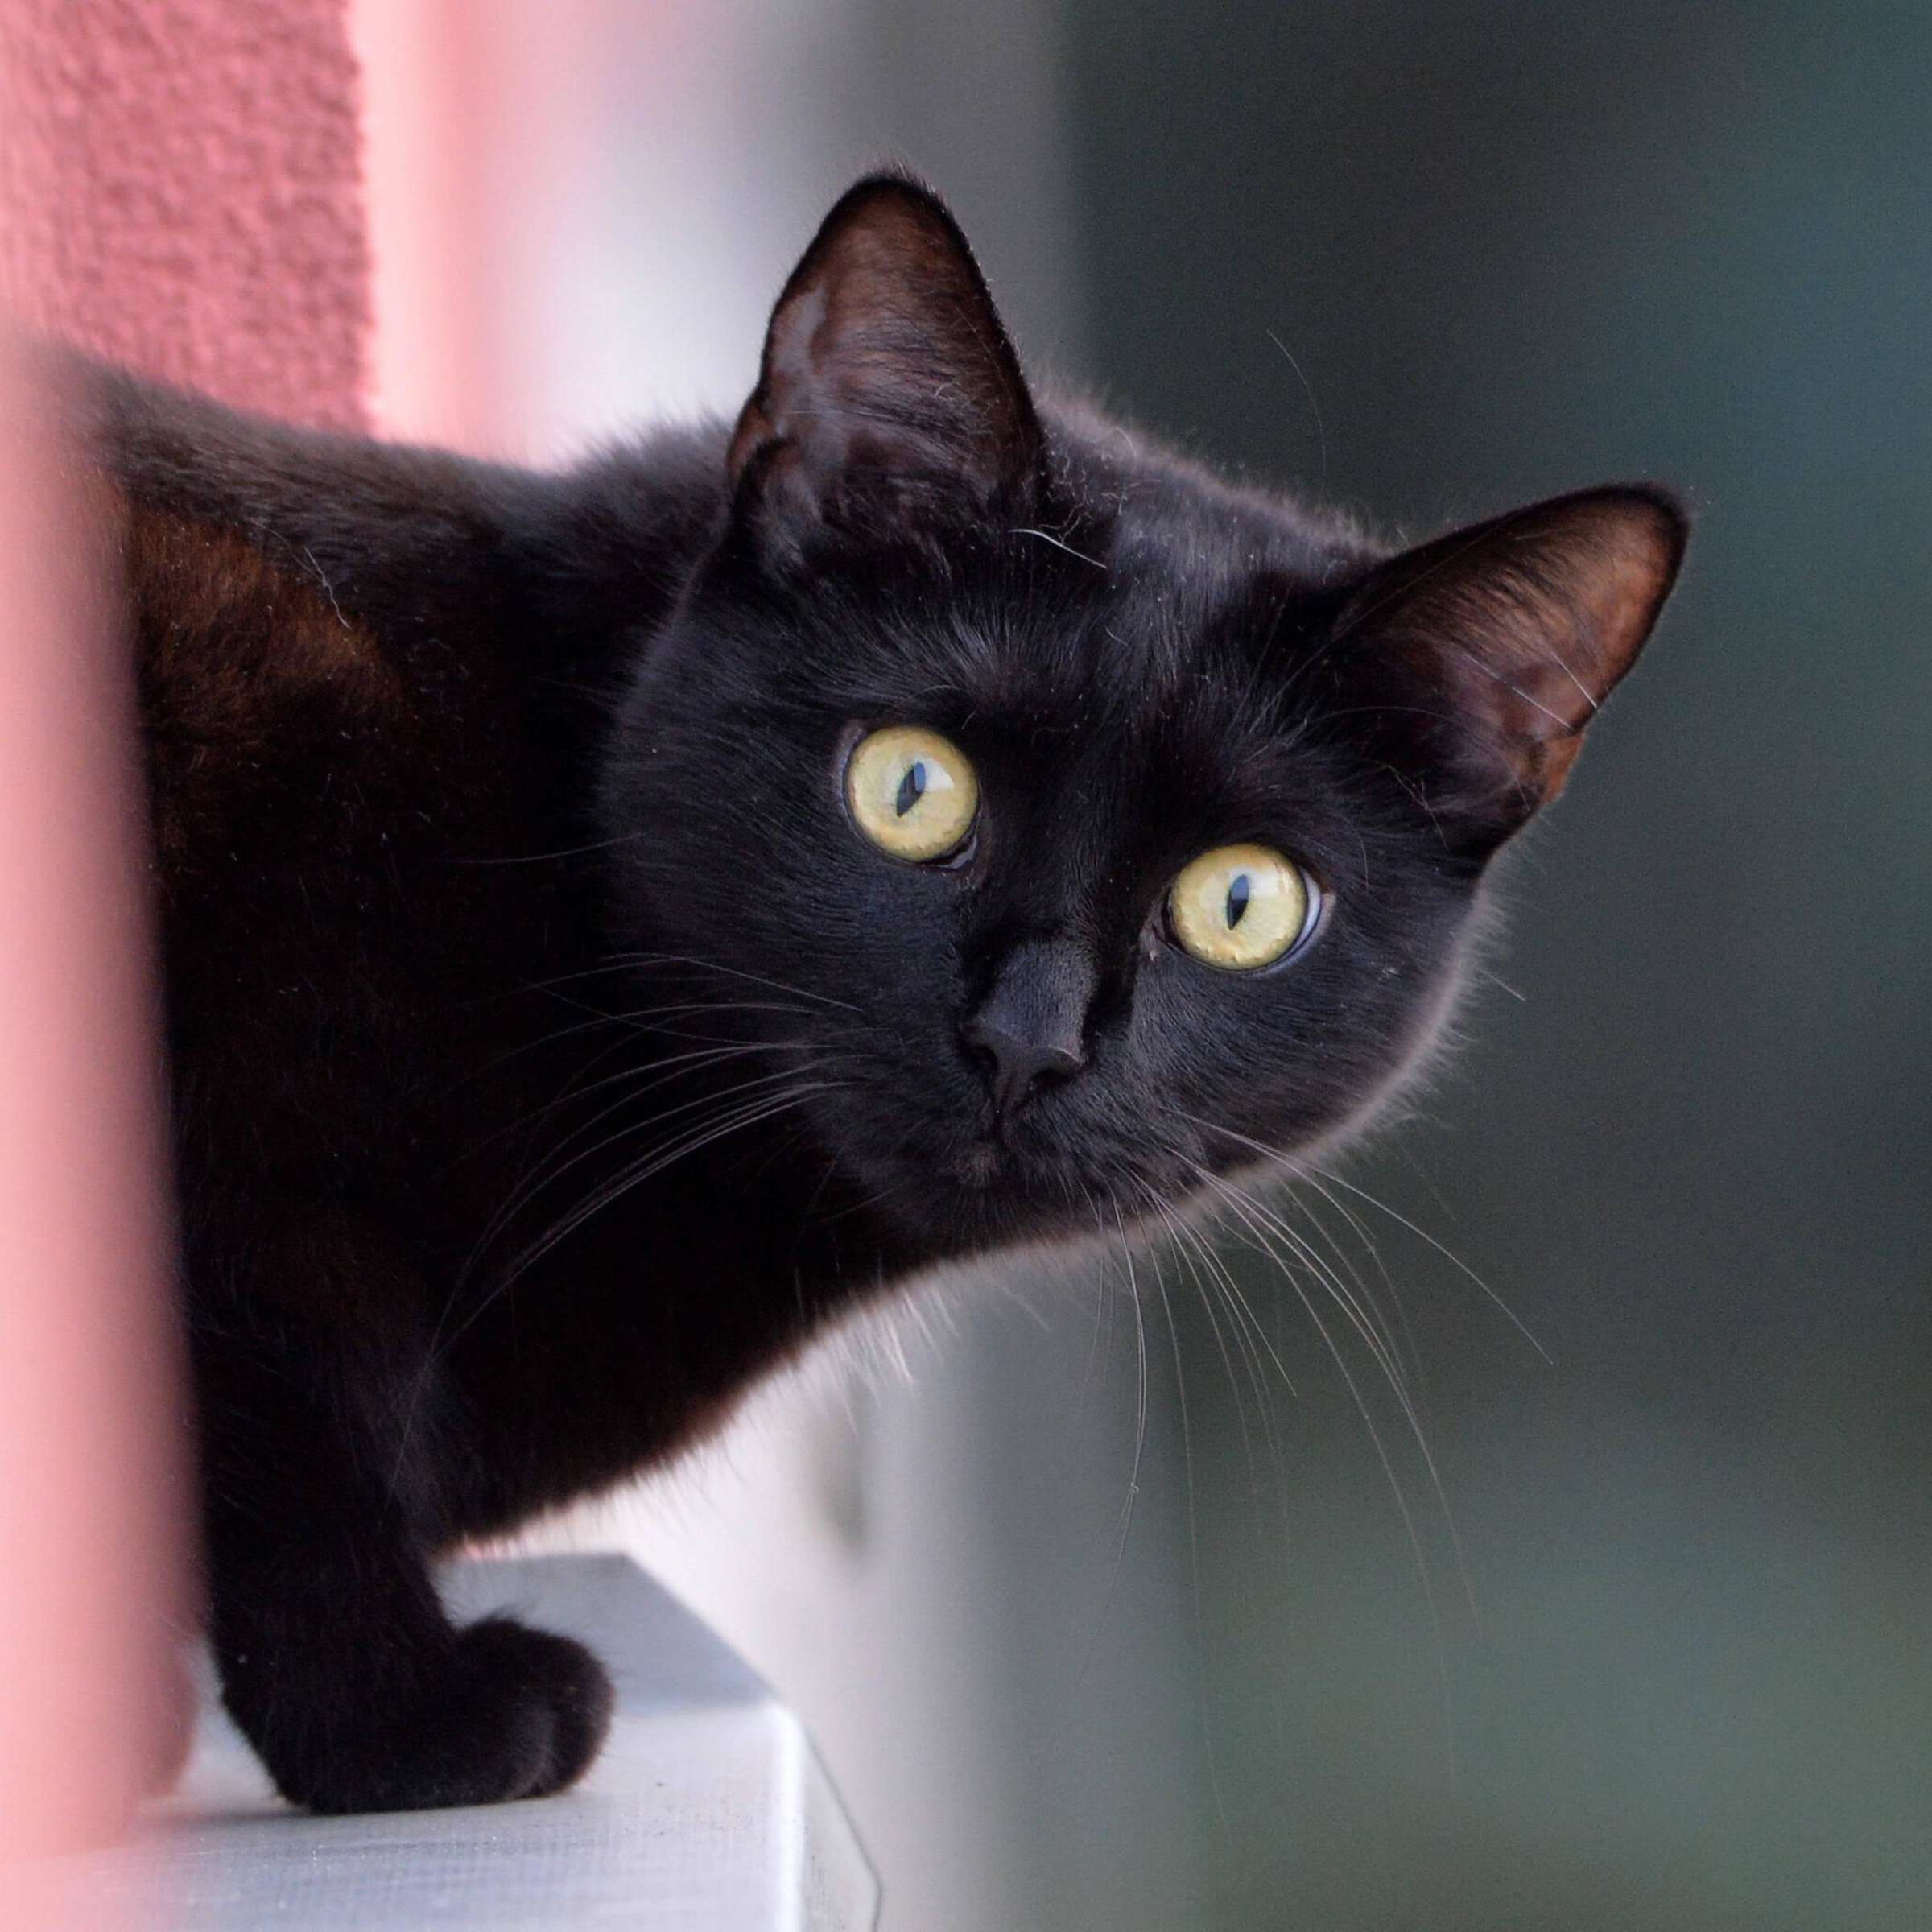
\includegraphics[width=0.5\linewidth, height=0.3\textheight]{./Abbildungen/Beispiel.jpg}
	\end{figure}	
	\newpage
	
	\section{Image mit Bildunterschrift}
	\begin{figure}[h!hbt]
		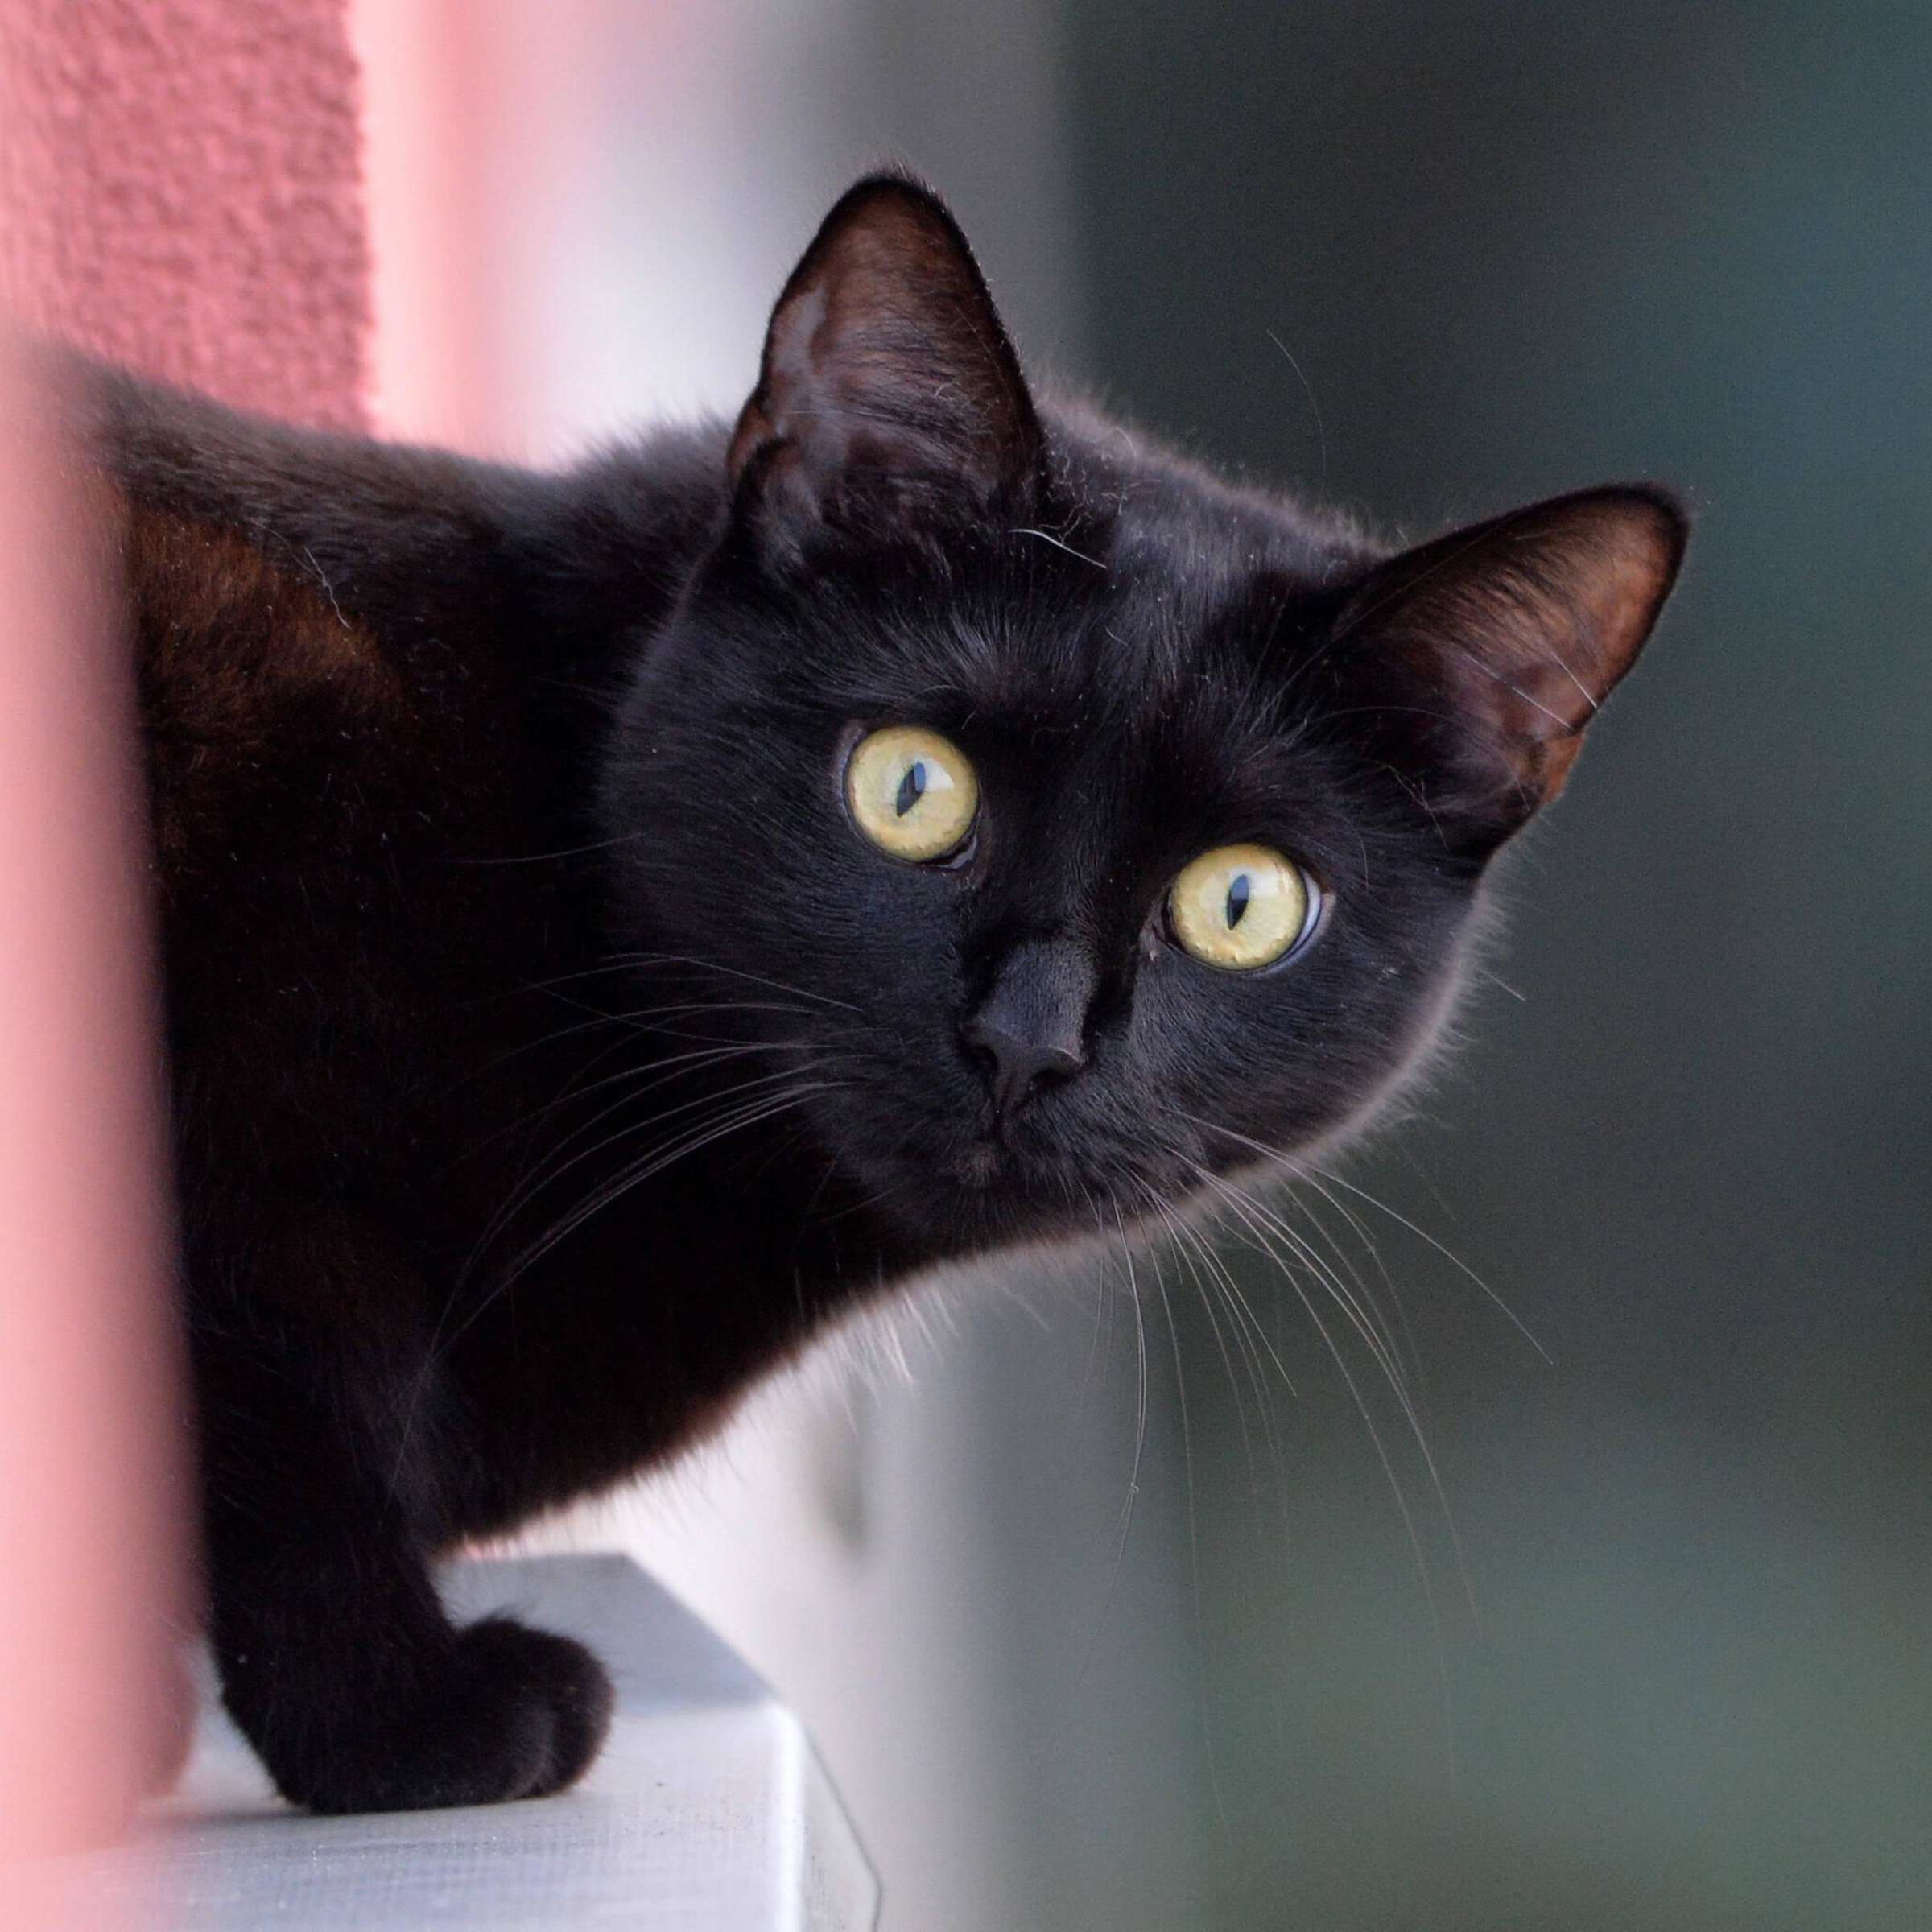
\includegraphics[width=\linewidth]{./Abbildungen/Beispiel.jpg}
		\caption{Beispielgraphik}
	\end{figure}
	\newpage
	
	\section{Image mit Label / Referenz}
	\begin{figure}[h!hbt]
		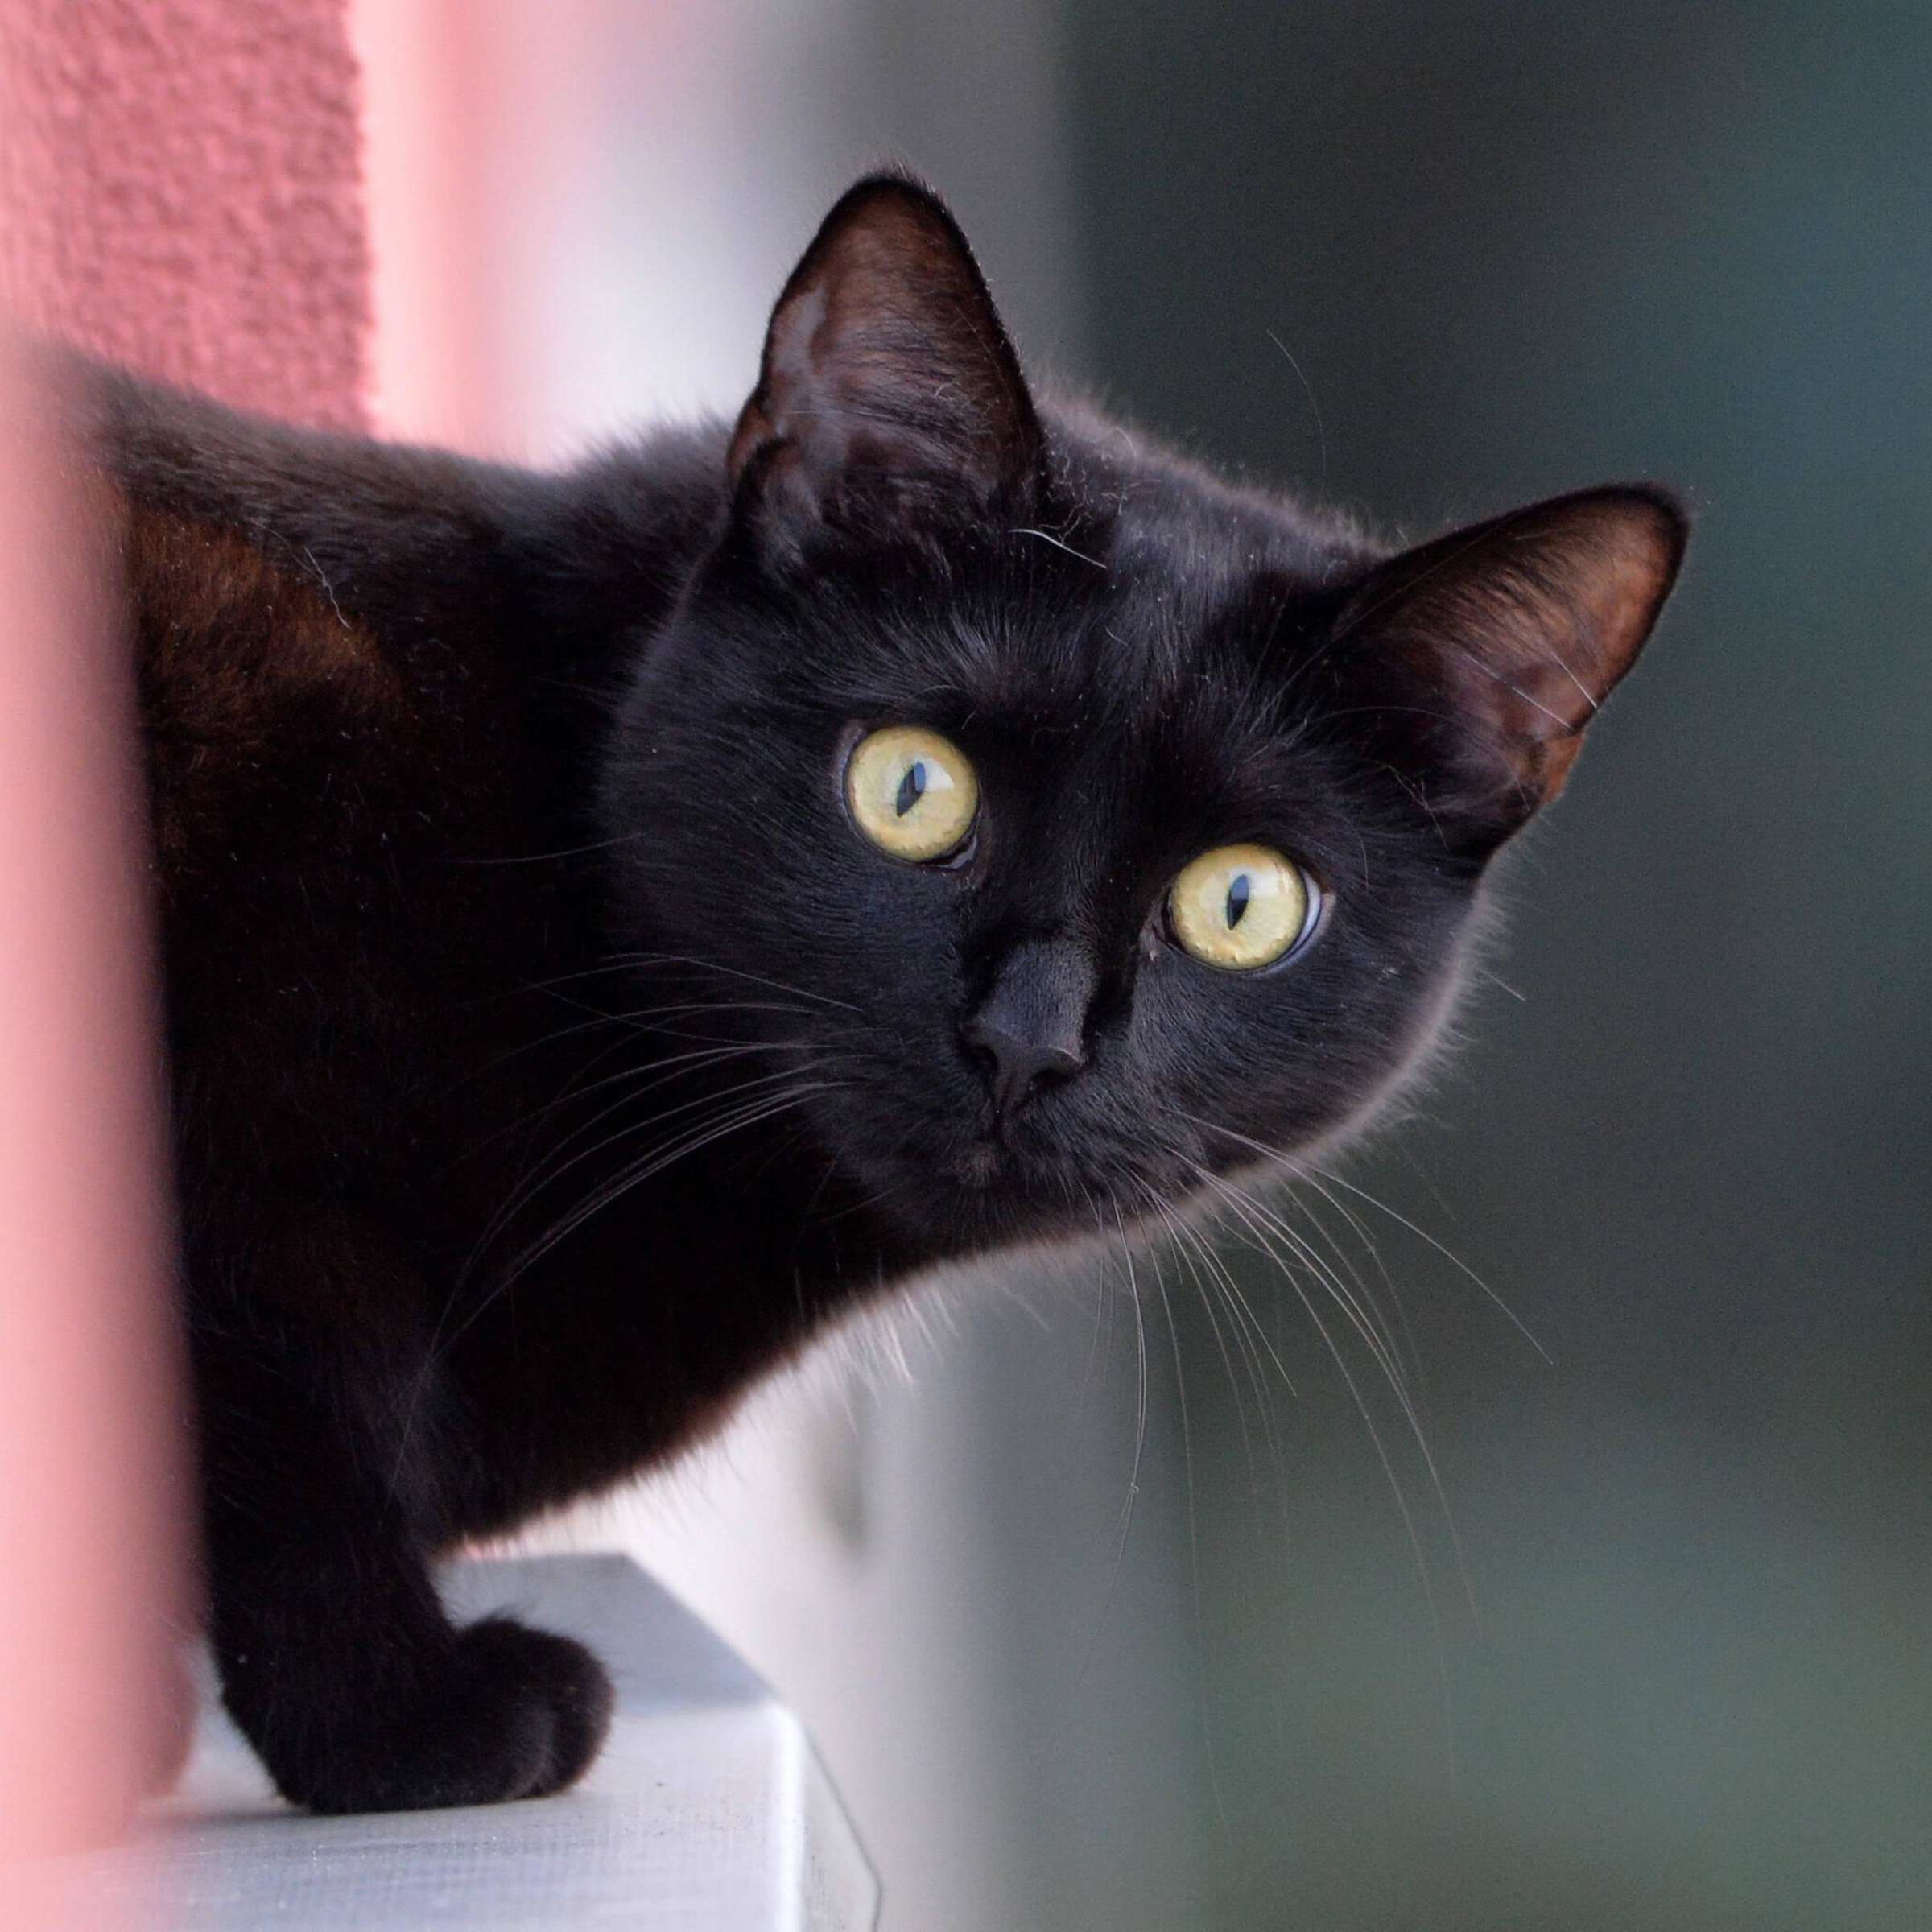
\includegraphics[width=\linewidth]{./Abbildungen/Beispiel.jpg}
		\label{Abb: Beispiel1} %Einzigartig pro Arbeit! Dadurch kann man eine Direkt-Referenz auf das Bild erstellen.
	\end{figure}
	\newpage
	
	\section{Zentriertes Image inkl. Label, Bildunterschrift und angepasste Größe}
	\begin{figure}[h!hbt]
		\centering
		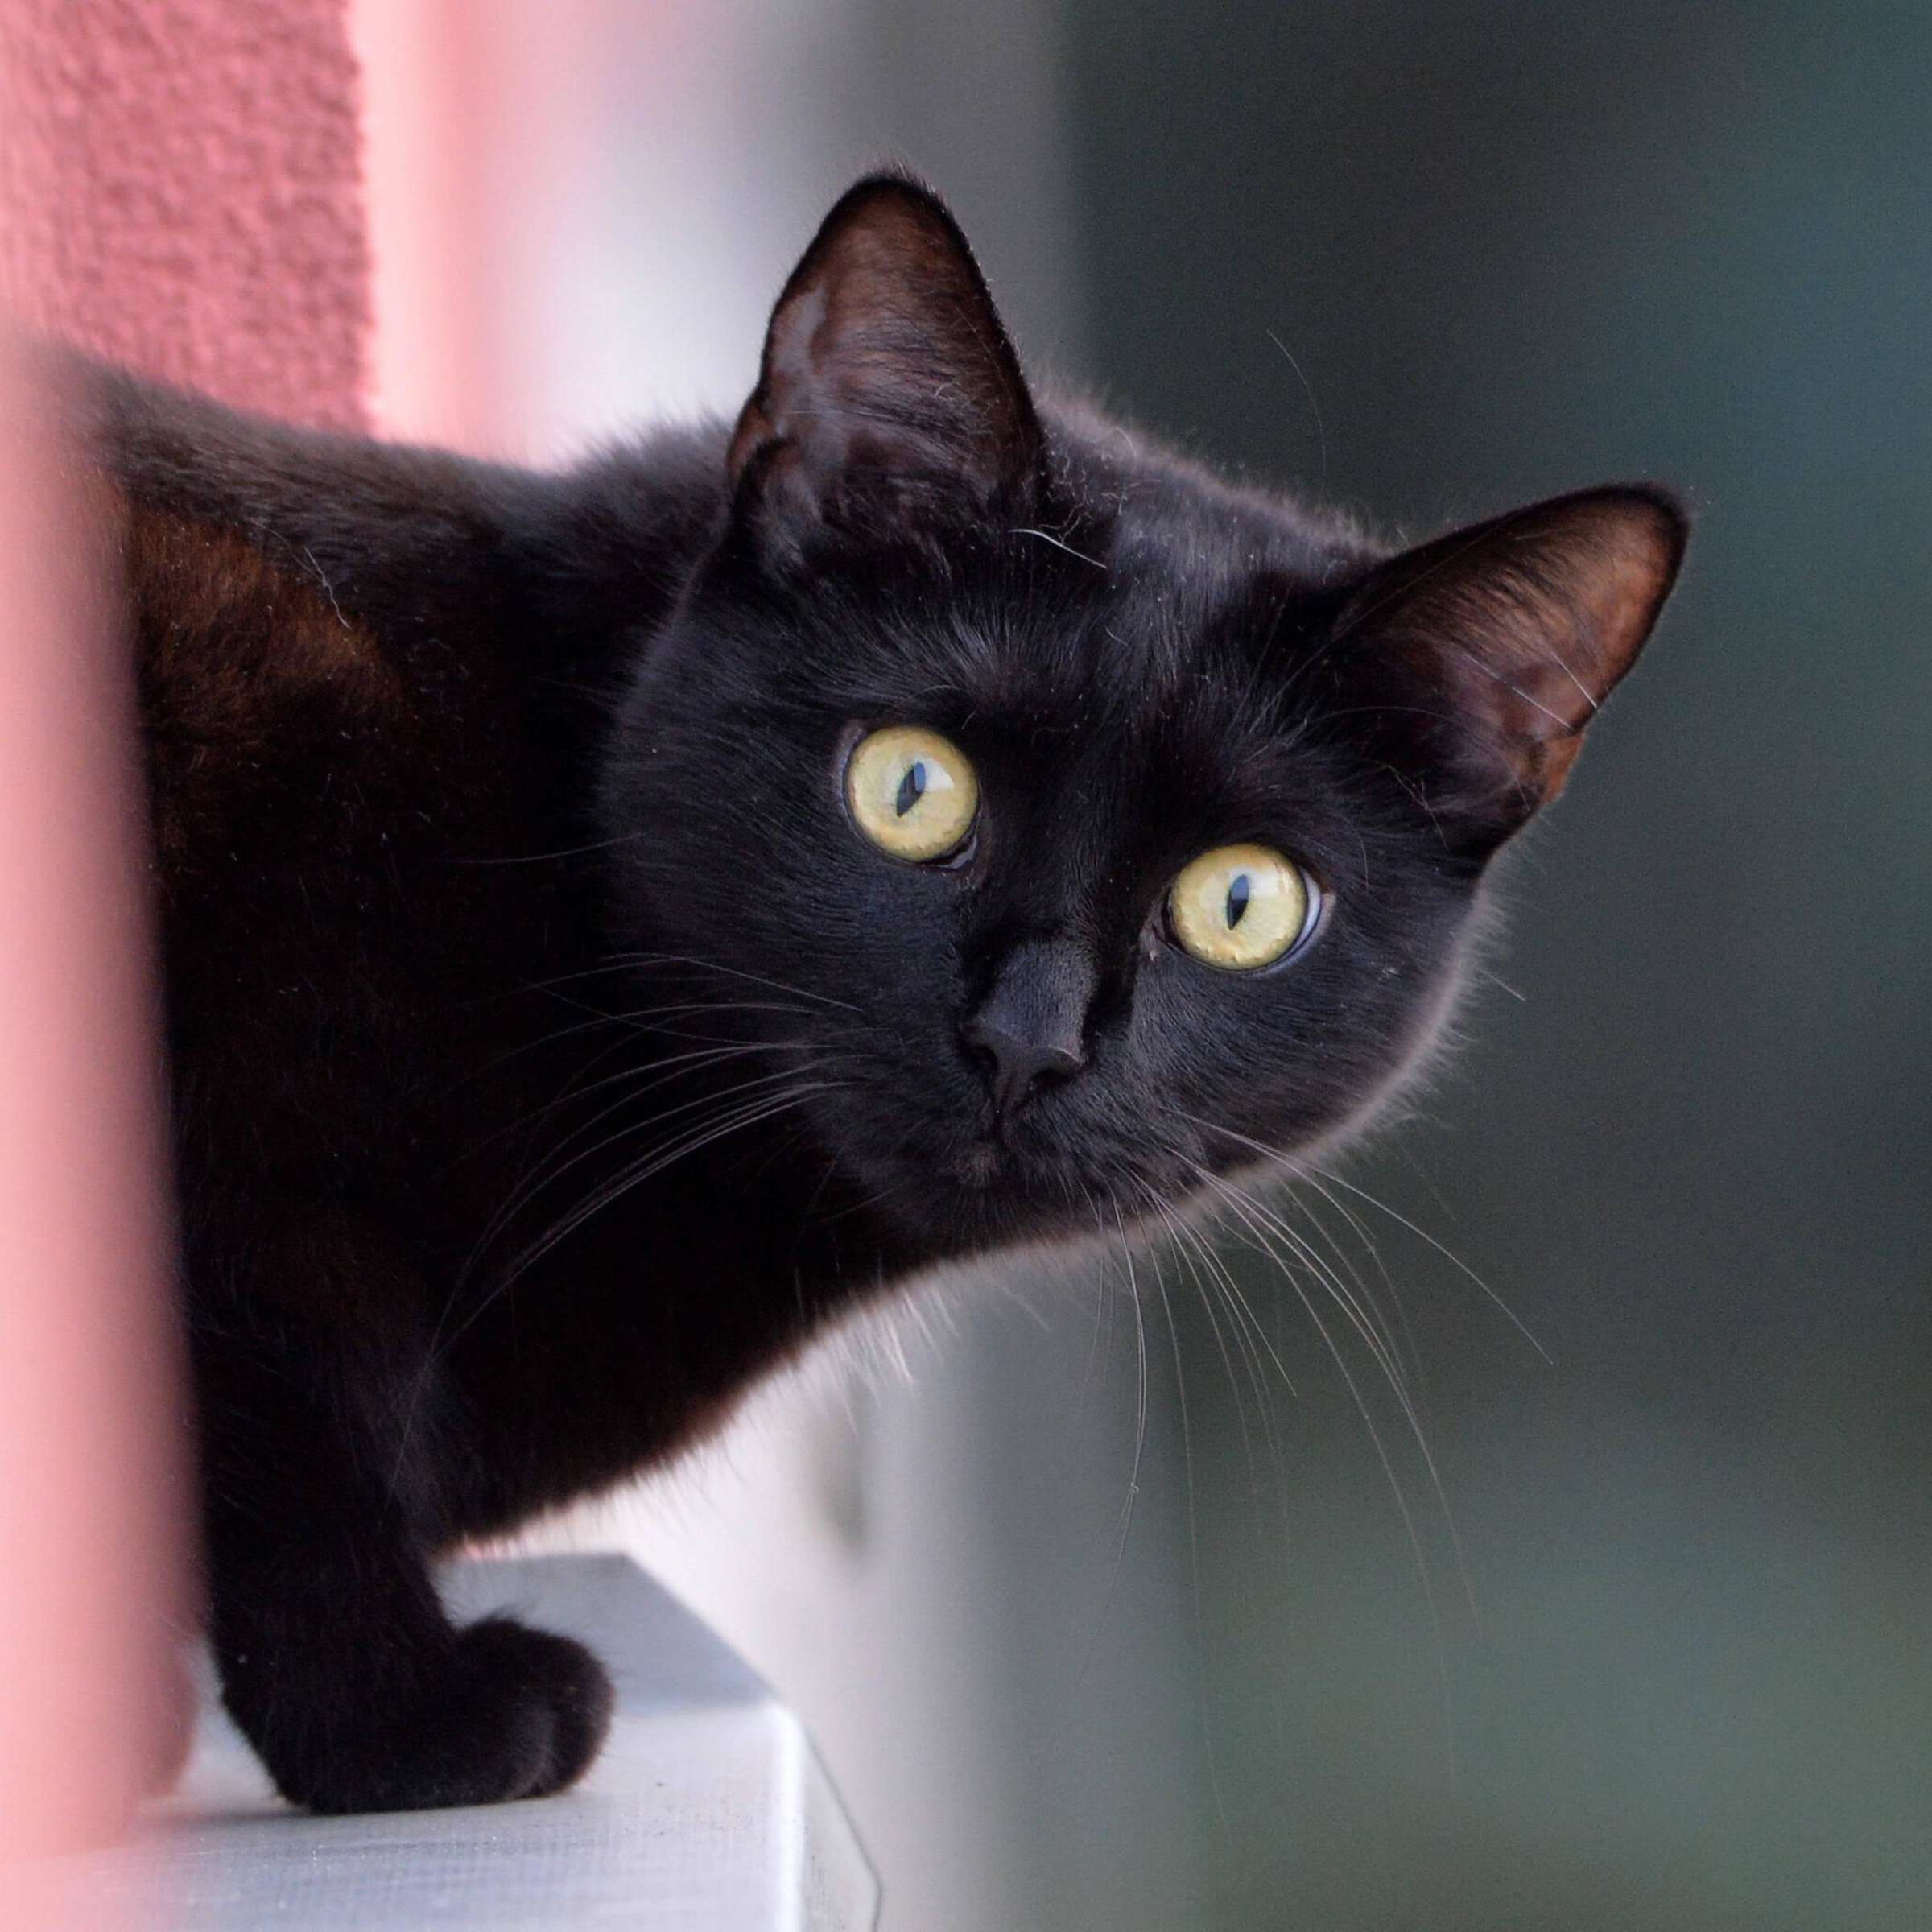
\includegraphics[width=0.8\linewidth]{./Abbildungen/Beispiel.jpg}
		\caption{Beispielgraphik}
		\label{Abb: Beispiel2}
	\end{figure}
	\newpage
	
	\section{Image mit Quellenangabe}
	\begin{figure}[h!hbt]
		\centering
		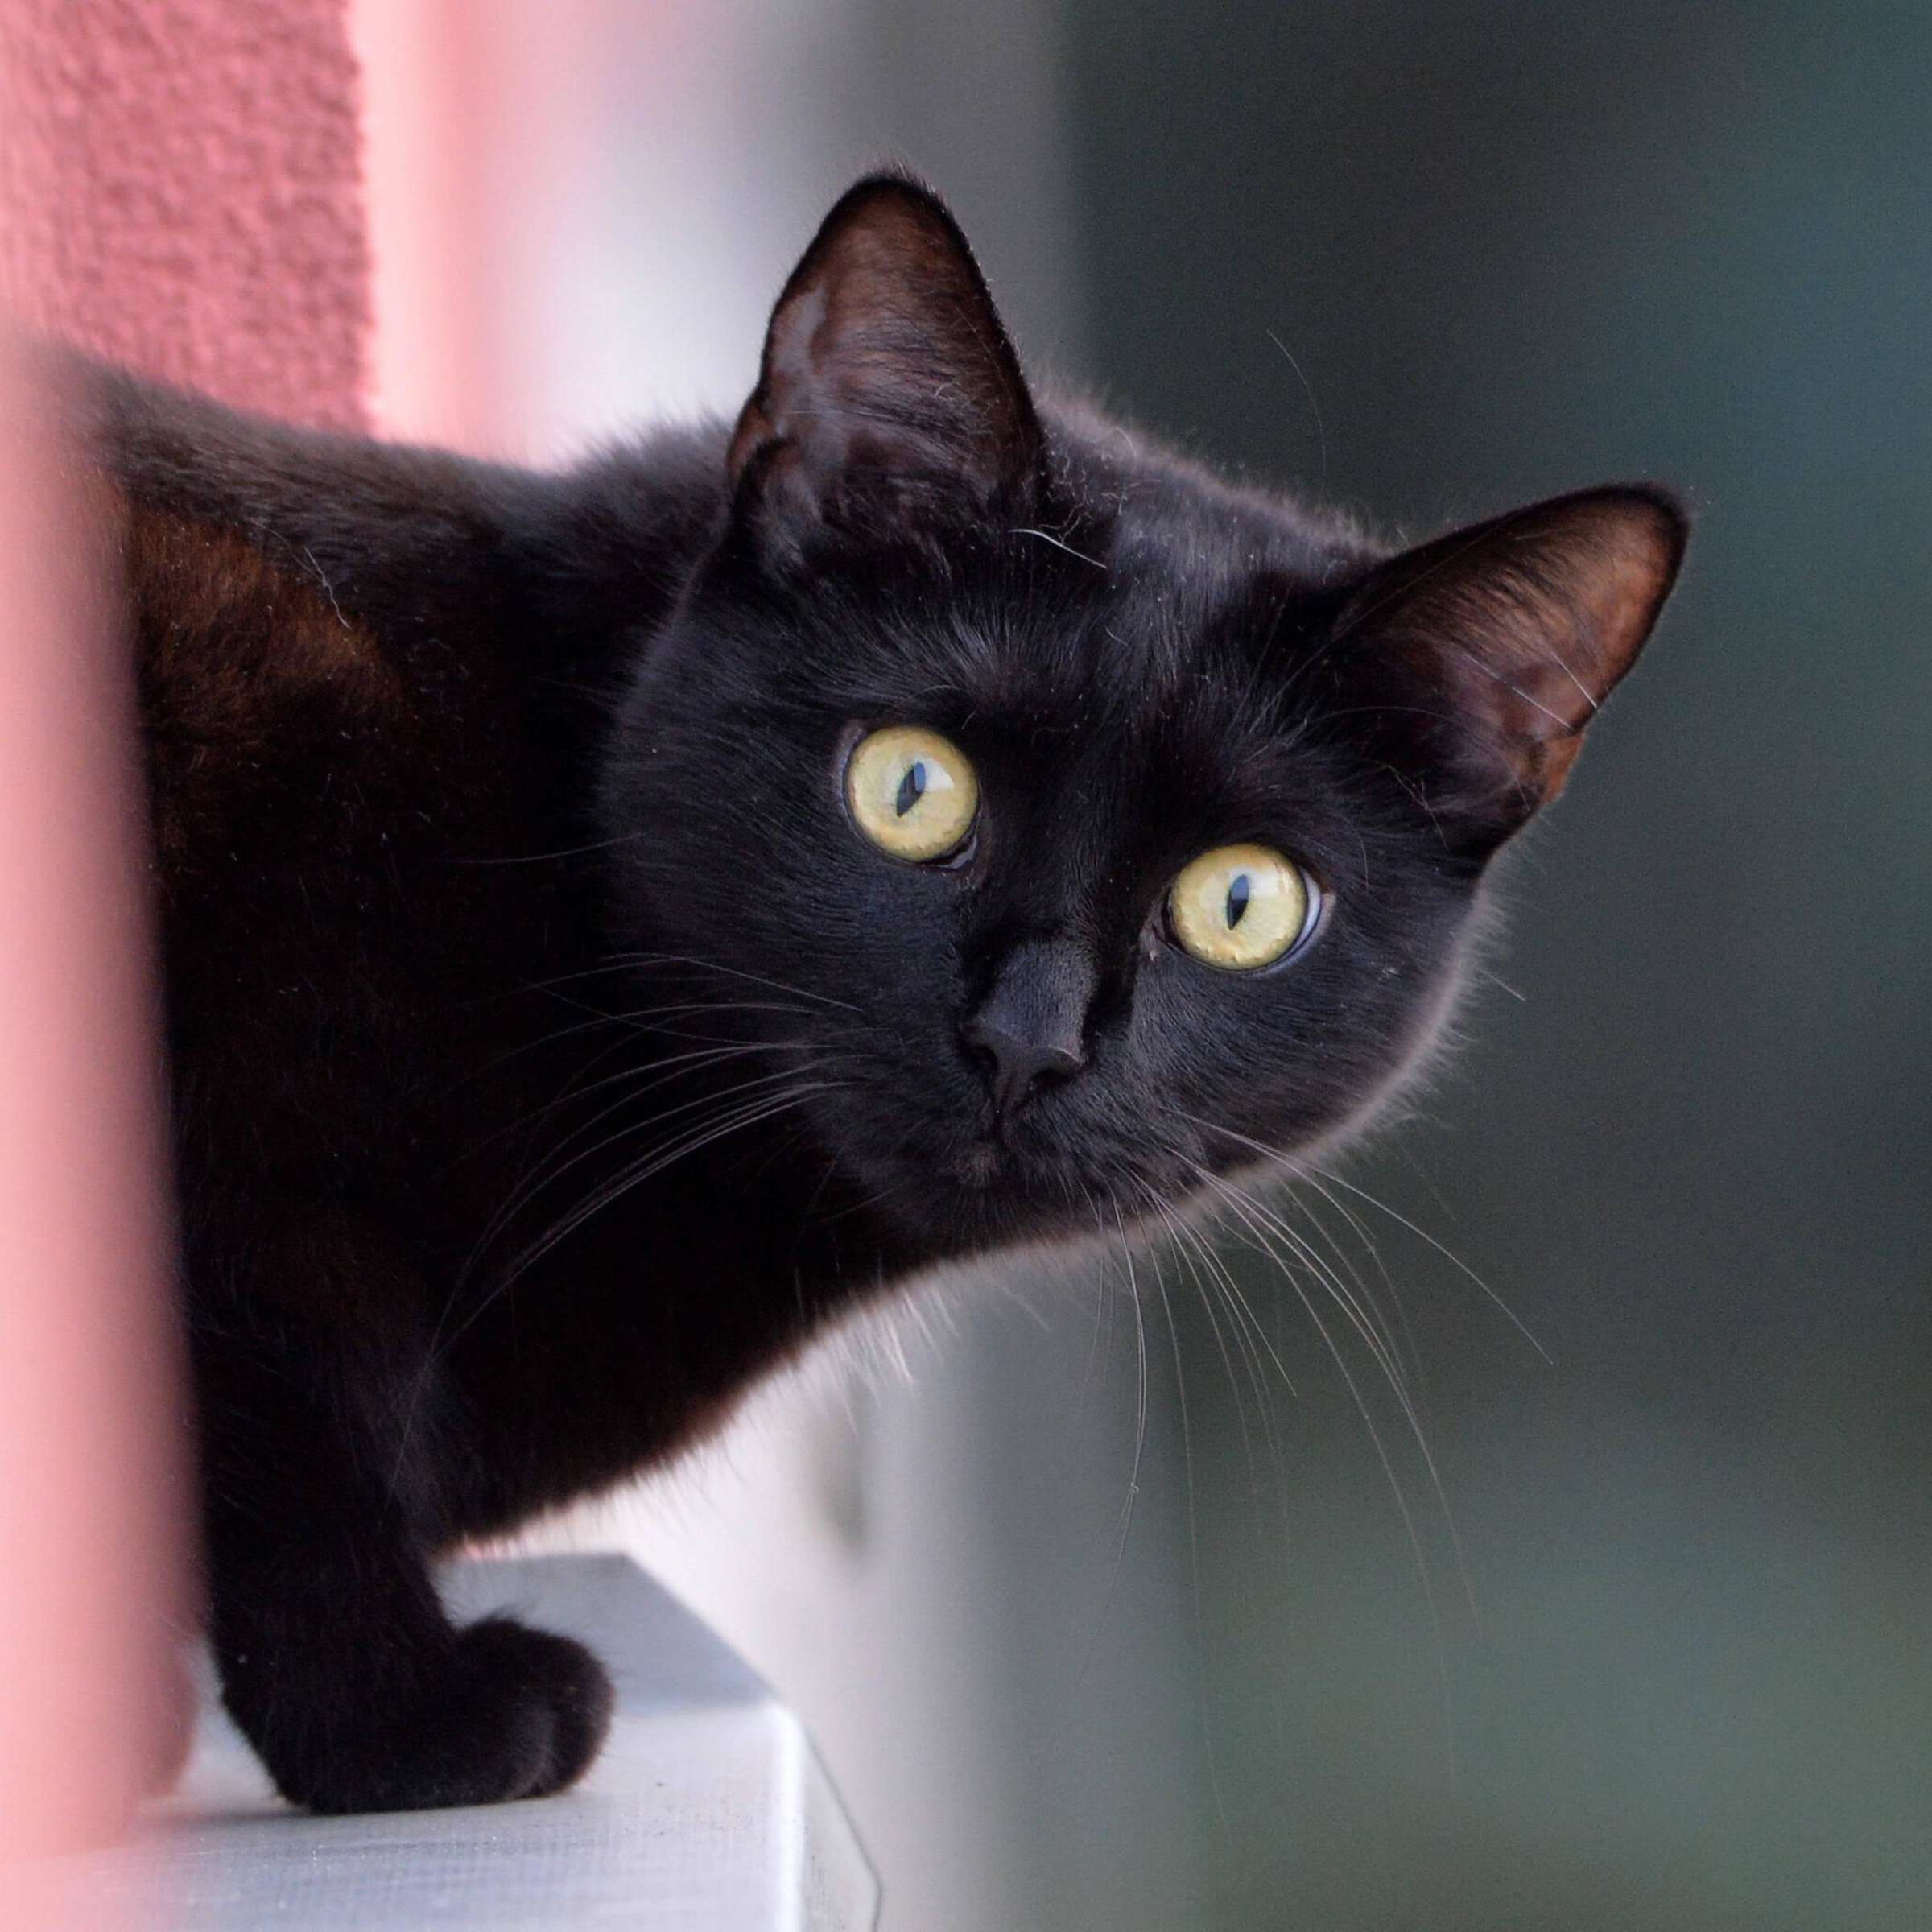
\includegraphics[width=\linewidth]{./Abbildungen/Beispiel.jpg}
		\raggedleft{\text{\footnotesize Quelle:\href{https://de.wikipedia.org/wiki/Hauskatze}{Wikipedia}
		}}
	\end{figure}
\end{document}
